% !TEX root = main.tex

In this section we detail the inventory, energy plus simulation methodology, important assumptions, and the LCA evaluation method. The assessment considers the environmental impacts of the production, operation, and disposal of an ASF. We assume a life time of 20 years based on the product warranty of the PV panels.
\\

\subsection{Life Cycle Inventory and Assumptions}

The mechanical components of the ASF can be broken into four parts: a PV panel, actuator, cantilever, and a cable net supporting structure. The PV panel, actuator and cantilever combine to form a dynamic PV module, which is then mounted on a cable net supporting structure. An exploded view of these components can be seen in Figure \ref{fig:explodedView}. There are also additional electronics which exists off the facade in a separate control box. Theses five components along with the assembly, are the main product systems in the manufacture of the ASF as seen in Figure \ref{fig:BOS}. 

\textcolor{magenta}{\textit{\\It is absolutely necessary that we describe the system boundary (what is included and what not (e.g. transport) and why) and also the functional unit! Were all life phases properly described? What happens in the maintenance, disposal phase? Will we have an annex? If so, we should give the ecoinvent inventories there.}}


% \begin{figure}[H]
% \begin{center}
% 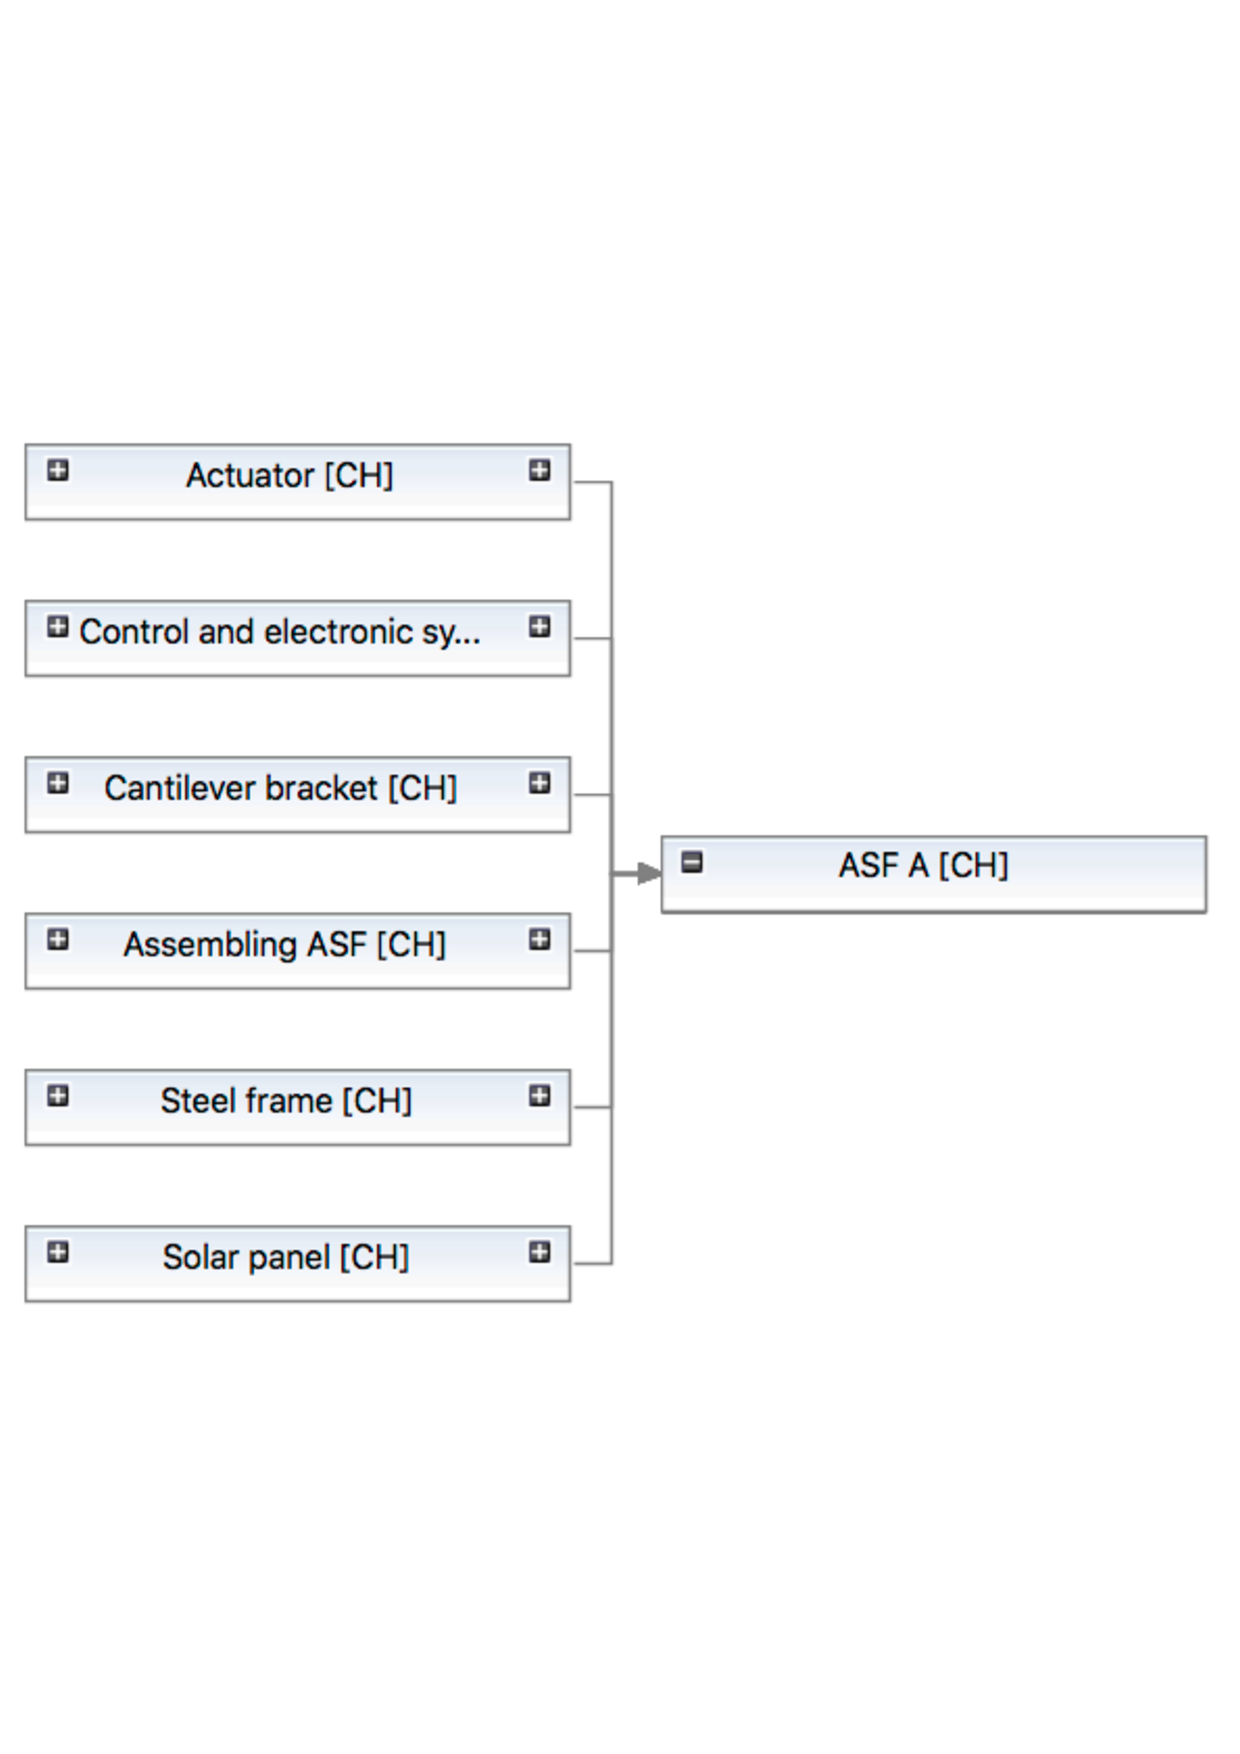
\includegraphics[width=8cm, trim= 0cm 0cm 0cm 0cm,clip]{ASFSubsystems.pdf}
% \caption{Breakdown of the ASF into six sub-product systems (Note change Steel frame to Suporting Structure, and Assembling ASF to Assembly. Also redraw this chart so it matches the subsubsections below)}
% \label{fig:subsystem}
% \end{center}
% \end{figure}

\begin{figure}[H]
\begin{center}
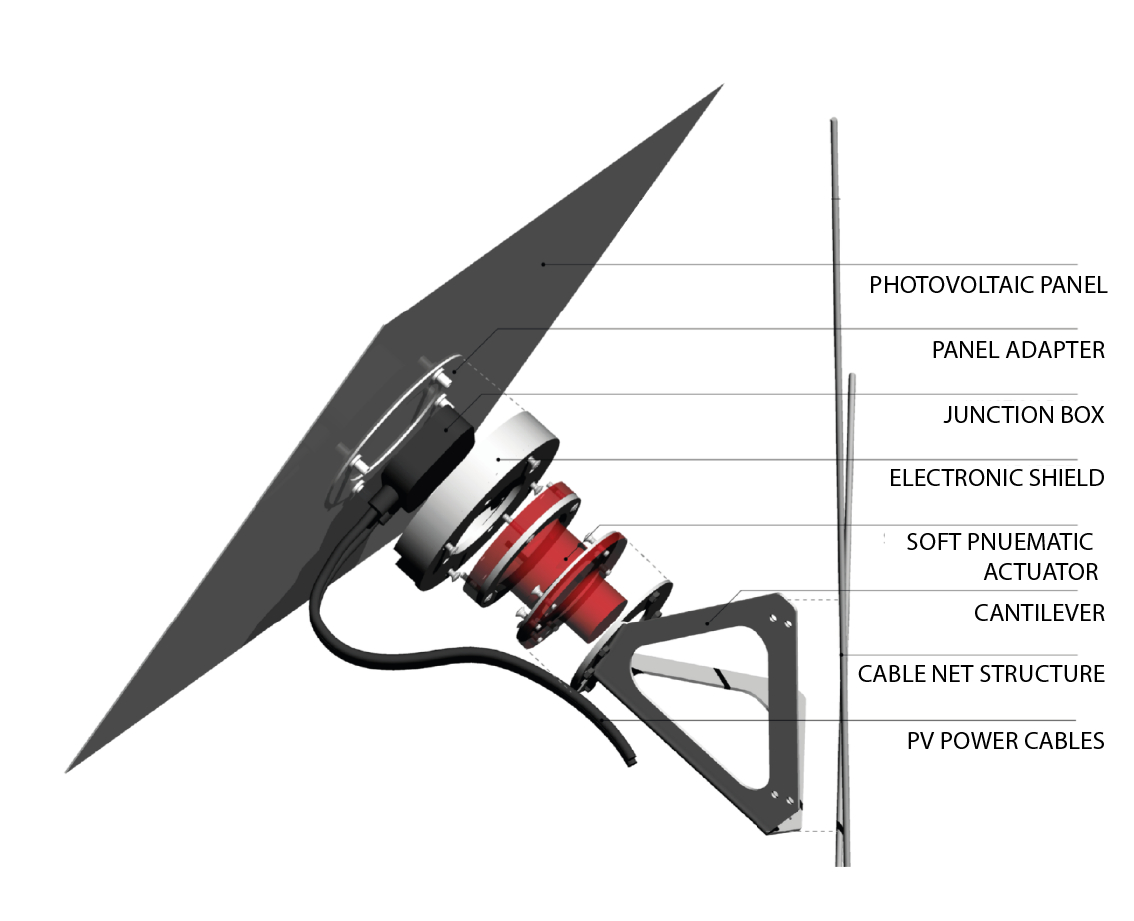
\includegraphics[width=8cm, trim= 0cm 0cm 0cm 0cm,clip]{explodedASFV2.png}
\caption{Exploded view of an ASF module mounted on a cable net supporting structure}
\label{fig:explodedView}
\end{center}
\end{figure}

\begin{figure}[ht]
\begin{center}
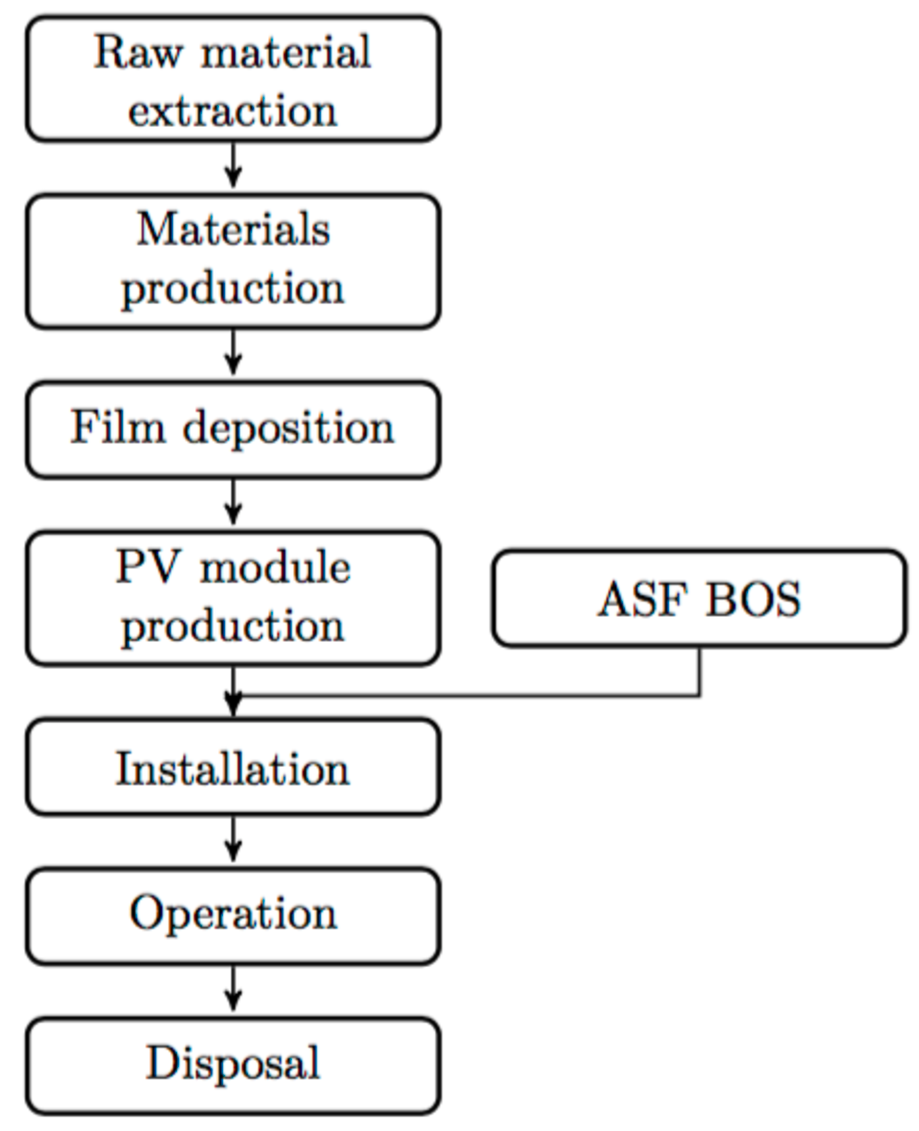
\includegraphics[width=14cm, trim= 0cm 0cm 0cm 0cm,clip]{BOS.pdf}
\caption{Breakdown of the ASF into five embodied product components and installation costs, operational costs, and disposal}

\label{fig:BOS}
\end{center}
\end{figure}
\textcolor{magenta}{\textit{(May Move the text to an Appendix and just keep the inventories)}}
\begin{description}

\item[PV Panel] \hfill\\
Weight is the primary restriction when selecting a PV panel. Any technology that requires glass encapsulation or a heavy substructure can therefore not be used. This limits us to CIGS and amorphous silicon panels.\\

CIGS PV panels was selected as the thin film panel of choice due to its high efficiency, low cost, and ability to be deposited on a polymer or aluminium substrate \cite{chirilua2011highly}. 

%A less efficient thin film amorphous silicon panel could also be used and will also be discussed in this analysis.\\

\textcolor{magenta}{\textit{(Not sure if it makes sense to provide the entire inventory here. If so, we would probably also need to give expected lifetimes, etc.)}}

% \begin{table}[H]
% \centering
% \begin{tabular}{lll}
% Panel Type  & SMQ    & ${\mathrm{\eta}}$  \\
% \hline
% CIGS 				& 0.7036 ${\mathrm{m^2_{panel}/m^2}}$ & \% \\
% a-Si				 	& 0.7036 ${\mathrm{m^2_{panel}/m^2}}$ & YY\%    \\
% Aluminum sheet 		& x ${\mathrm{kg/m^2}}$
% \end{tabular}
% \caption{Possible PV technologies for an ASF [Ref required]}
% \label{tab:PV}
% \end{table}

\begin{table}[H]
\centering
\begin{tabular}{ll}
\hline
Material description & SMQ \\ \hline
CIGS PV film       	 & 0.569 ${\mathrm{m^2_{PV}/m^2_{facade}}}$\\
Aluminum sheet 	 & 1.593 ${\mathrm{kg/m^2_{facade}}}$\\
Chromium steel panel adapter  & 1.422 ${\mathrm{kg/m^2_{facade}}}$\\
Polyethylene for junction box & 0.036 ${\mathrm{kg/m^2_{facade}}}$\\
Diode, glass for junction box & 0.011 ${\mathrm{kg/m^2_{facade}}}$\\
\hline
\end{tabular}
\caption{Inventory of a selection of top five input flows to the PV manufacturing process [ref required]}
\label{tab:PVinv}
\end{table}

\item[Actuator] \hfill \\
Traditionally photovoltaic actuation is done through the use of servo motors. Servo motors however become a limiting factor for adaptive facades due to their high upfront costs, and instability in heavy winds. Soft robotic actuators on the other hand are cheaper and more resilient to harsh environmental conditions\cite{Svetozarevic2014a}. The soft robotic actuators however are still in development and have a life time of five years. They will therefore require two rounds of maintenance during the lifetime of the ASF.
For the purpose of this analysis we will analyse both servo motors and soft robotic actuators. 

\begin{table}[H]
\centering
\begin{tabular}{ll}
\hline
Material description & SMQ \\ \hline
Chromium steel rings	 & 1.0665 ${\mathrm{kg/m^2_{facade}}}$ \\
Electronics, for control, 2-2way valves  & 0.0130  ${\mathrm{kg/m^2_{facade}}}$\\
Silicone chambers & 0.8887 ${\mathrm{kg/m^2_{facade}}}$\\
Polyurethane tubes &0.0933 ${\mathrm{kg/m^2_{facade}}}$\\
Air compressor, screw type, 0.75kW & NA ${\mathrm{kg/m^2_{facade}}}$\\
\hline
\end{tabular}
\caption{Inventory of four main input flows to the Actuator manufacturing process [ref required]}
\label{tab:ActuatorInv}
\end{table}

\item[Cantilever] \hfill \\
The cantilever is a steel connection point between the PV panel and the supporting structure.\\

\begin{table}[H]
\centering
\begin{tabular}{ll}
\hline
Material description & SMQ \\ \hline
Chromium steel bracket	 & 1.4220 ${\mathrm{kg/m^2_{facade}}}$ \\
Chromium steel fixing clamp  & 0.0284 ${\mathrm{kg/m^2_{facade}}}$\\
\hline
\end{tabular}
\caption{Inventory of main input flows to the Cantilever manufacturing process [ref required]}
\label{tab:CantileverInv}
\end{table}

\item[Supporting Structure] \hfill \\
The supporting structure is the connection point between the array of photovoltaic modules and the building itself. Many different designs are possible, however we will base our analysis of an adaptive solar facade that has already been constructed \cite{nagy2015frontiers}. This design consists of a steel cable-net that spans a steel supporting frame. The steel frame is then attached to the building itself.\\

\begin{table}[H]
\centering
\begin{tabular}{ll}
\hline
Material description & SMQ \\ \hline
Chromium steel L bar	 & 4.2581 ${\mathrm{kg/m^2_{facade}}}$ \\
Chromium steel U bar  & 2.7347 ${\mathrm{kg/m^2_{facade}}}$\\
Chromium steel swaged external thread  &0.2897 ${\mathrm{kg/m^2_{facade}}}$\\
Chromium steel wire rope WC  & 0.1593 ${\mathrm{kg/m^2_{facade}}}$\\
\hline
\end{tabular}
\caption{Inventory of the four main input flows to the manufacturing process of the Supporting Structure[ref required] \textcolor{cyan}{Could we change the L bar and U bar to Chromium Steel Frame? It is easier to understand}}
\label{tab:StructureInv}
\end{table}

\item[Control System and Electronics] \hfill \\
The control system is required for the actuation of panels and the regulation of photovoltaic electricity production.\\

\begin{table}[H]
\centering
\begin{tabular}{ll}
\hline
Material description & SMQ \\ \hline
Inverter 1.25kW	 & NA ${\mathrm{kg/m^2_{facade}}}$ \\
PV cable  & 3.1995 ${\mathrm{kg/m^2_{facade}}}$\\
Electronics control\footnote{c-Rio,8-slot, integrated 667Mhz}& 0.0419 ${\mathrm{kg/m^2_{facade}}}$\\
Electronics control\footnote{NI9476 32ch DO with cables and connectors}& 0.0097${\mathrm{kg/m^2_{facade}}}$\\
\hline
\end{tabular}
\caption{Inventory of the four main input flows to the manufacturing process of the Control System[ref required]}
\label{tab:ControlInv}
\end{table}

\item[Assembly] \hfill \\
There are many assembly options available. From past experience, an installation of an equivalent ASF required a hydraulic hoist which was in operation for eight hours \cite{jayathissa2015abs}. \\

\begin{table}[H]
\centering
\begin{tabular}{ll}
\hline
Material description & SMQ \\ \hline
Hoist, diesel  ${<}$18.64kW idling 8 hours & \textcolor{red}{NA} ${\mathrm{kg/m^2_{facade}}}$ \\
\hline
\end{tabular}
\caption{Inventory of main input flows to the Assembly Process[ref required] \textcolor{cyan}{Note that the 8 hours was for the HoNR ASF. We can scale this to get a value per sqm}}
\label{tab:AssemblyInv}
\end{table}

\end{description}

\subsection{Operational Emissions and Assumptions}
\label{ch:Meth:Opp}

The potential savings are based off previously completed numerical simulations \cite{jayathissa2015abs}. The simulation was conducted on a south facing office room. The room 7.0 meters in length, 4.9 meters wide and 3.1 meters high was modeled using Rhinoceros 3D CAD Package \cite{Rhino}. Grasshopper \cite{grasshopper} was used to model the orientation of each photovoltaic panel. The geometrical input is imported to Energy Plus \cite{energyplus} though the DIVA \cite{DIVA} interface. A single zone thermal analysis was conducted for each possible geometrical configuration of the ASF for each hour of the year. \textcolor{magenta}{(\textit{I don't get it. You couldn't simulate one hour only - that would contradict dynamic modelling ;D})} The results were then post processed in Python \cite{python} with the NumPy \cite{numpy}, and Pandas \cite{pandas} packages.\\

We conducted the simulation for three scenarios: 1) facade with no shading, 2) a facade with a static shading system angled at 45$^{\circ}$ to the horizontal axis, and 3) an adaptive solar facade \cite{jayathissa2015abs}. This analysis purely looks at the building energy performance through adaptive shading and doesn't include electricity production from the photovoltaic panels.\\

The energy consumption (in kWh), due to reduced cooling load, heating, and lighting is compared to a base case with no external shading. This difference is converted to a GWP value based on the emission factor of the European Network of Transmission System Operators for Electricity (ENTSO-E) electricity mix (gCO2/kWh) \textcolor{blue}{[Add value and reference]}.\textcolor{magenta}{\textit{(Not sure what MJ used, but we could use the 0.4594 kg CO2-eq / kWh, I calculated for my paper http://dx.doi.org/10.1021/acs.est.5b01735)}} \\

The energy required for actuation is also taken into account. It takes \textcolor{red}{1.45Wh} to fully open a single actuator. Based on the assumption of four full openings and closings per day, we approximate the energy requirement to be 2286kWh in its 20 year lifetime. 
%However as seen in Section \ref{ch:results}, this has a \textcolor{magenta}{\sout{very} relatively} small impact.\\

\begin{table}[H]
\centering
\begin{tabular}{ll}
\hline
\textbf{Building Settings}    &                                                \\
Office Envelope               & Roof: Adiabatic                                \\
                              & Floor: Adiabatic                               \\
                              & Walls: Adiabatic                               \\
                              & Window: Double Glazed LoE (e=0.2) 3mm/13mm air \\
Thermal Set Points            & Heating: 22$^{\circ}$ degrees Celcius          \\
                              & Cooling: 26$^{\circ}$ degrees Celcius          \\
Building System               & Hydronic Heating: COP=4                        \\
                              & Hydronic Cooling: COP=3                        \\
Lighting Control              & Lighting set point: 11.8W/m2                   \\
                              & Lighting Control: 300 lx Threshhold            \\
                              & LED Lighting                                   \\
Occupancy                     & Office: Weekdays from 8:00-18:00               \\
                              & People set point: 0.1 persons/m2               \\
                              & Infiltration: 0.5 per hour                     \\
                              &                                                \\
\textbf{Location Assumptions} &                                                \\
Weather File                  & Geneva, Switzerland (067000IWEC)               \\
Electricity Mix               & ENTSO-E \cite{itten2012life}                   \\
                              &                                                \\
\textbf{Maintenance}          &                                                \\
Actuator Changes              & Every 5 years                                  \\
                              &                                                \\
\textbf{ASF Settings}         &                                                \\
Full open and closes per day  & 4 per day                                      \\
\hline
\end{tabular}
\caption{Summary of main assumptions for the calculation of operational emissions \textcolor{magenta}{\textit{What thermal resistance? Maybe give surface areas}}}
\label{tab:AssumptionsOpp}
\end{table}


% Maybe have a reference case here, see previous commits 

\subsection{Evaluation Method}
The life cycle analysis is performed according to the ISO 14040 and ISO 14044 and is performed in five stages 1) goal, 2) scope definition, 3) inventory analysis, 4) impact assessment and 5) interpretation. We discuss these stages in the following. % 15804 to be discussed

\begin{description}
\item[1. Goal] This paper assesses carbon emission reductions, therefore the impact category used is the global warming potential (GWP\textcolor{magenta}{\textit{[IPCC 2013 reference - let me know if you need it]}}). This analysis will also touch on the regional distributions of GWP and terrestrial acidification to give a complete picture.


\item[2. Scope] The scope of the assessment is sumarised in Figure \ref{fig:BOS}. We analyse the GWP of embodied carbon, dynamic actuation, maintenance, disposal and the GWP savings through adaptive shading. 


% The GWP is computed as
% \begin{equation}
% \sum GWP={\mathrm{GWP_{Em}  + GWP_{Act} + GWP_{M} + GWP_{Disp} - GWP_{Opp} }},
% \label{eq:GWP}
% \end{equation}
% where $GWP_{Em}$ is the Embodied Energy, $GWP_{Act}$ is the Dynamic Actuation, $GWP_{M}$ is Maintenance, and $GWP_{Disp}$ is Disposal. The GWP savings through adaptive shading $GWP_{Opp}$ are subtracted to produce our final GWP. This scope is summarised in Figure \ref{fig:BOS}. 
\textcolor{magenta}{\textit{This is a little confusing. The reader doesn't know yet how to get from a piece of metal to CO2.}}
%\textcolor{red}{\textit{What does the sum sign refer to? This does not make sense to me. It should be GWP = ... // Also, why are those terms in uppercase?}}

% The functional unit needs to be based on the primary function of the technology. For adaptive building integrated photovoltaics this function can be twofold. When the adaptive BIPV acts as a shading system in front of a glass facade area the functional unit of ${\mathrm{m^2}}$ is used, while a comparison with static facade mounted photovoltaic systems requires the functional unit of electricity produced in ${\mathrm{kWh}}$. \textcolor{magenta}{\textit{(We should discuss the functional unit again. It should be defined more precisely / comprehensively.)}}



% In our assessment, we want to obtain the emission factor (gCO$_2$/kWh) of an ASF as expressed in Equation \ref{eq:EF}. 




% The electricity production, G, in kWh is expressed as
% \begin{equation}
% G=\frac{{\mathrm{GWP}}}{{\mathrm{I \cdot \eta  \cdot PR \cdot LT \cdot A}}}
% % what is G
% \label{eq:solar}
% \end{equation}
% based on [REF REQUIRED]. In~(\ref{eq:solar}) \textit{I} is the Irradiation \textcolor{red}{(unit)}, ${\eta}$ is the conversion efficiency, \textit{PR} is the performance ratio, \textit{LT} is the service life \textcolor{red}{(unit)}, and \textit{A} is the module area \textcolor{red}{(unit)}.
% \textcolor{red}{\textit{I rewrote this a little bit. You should try to a) make the equations part of the text, and b) the way you use the variables in the text should be the same as in the equations. Now you have I in italics in the text but as textrm in the actual equation. If you add the amsmath package you can use $\backslash$eqref to reference equations directly.\\
% Also why is G even used in this paragraph?}}


% The scope of the LCA comprises of the embodied, operational, and disposal global warming impact of the respective system. Figure \ref{fig:BOS} illustrates the system boundaries of the process flows. The supporting structures are also included in the system boundaries. The reason for this is that technologies within the building envelope also change the design of the supporting structures. The supporting structure of solar panels is referred to as balance of systems (BOS).\\

\item[3. Inventory] The inventory data was obtained from technical drawings, research papers describing the technology and expert judgement. The Ecoinvent v3.1 database is used as the main LCI database \cite{frischknecht2005ecoinvent}. To keep assumptions consistent, only data from this database is used. \textcolor{magenta}{\textit{(Is that so? Didn't we add a CIGS dataset?)}} Furthermore, the cut-off approach is used for the allocation of recycling and landfill disposal. This means that recycling does not generate any credit for the product and resulting benefits are not taken into account. Furthermore the use of recycled products do not bear the burden of processes higher up the chain.\textcolor{magenta}{\textit{(We don't do any system expansion??)}}\\



\item[4. GWP Assessment] For the assessment the ReciPe midpoint (H) indicator is used \cite{zelm2009recipe}. \textcolor{magenta}{\textit{Now that I read through it: We are not giving any Recipe result?????}} The GWP assessment is performed using the OpenLCA impact assessment tool \cite{ciroth2007ict}. The results of the assessment will be compared with the emission factor of other PV systems \cite{raugei2007life}\\
	% we may need to discuss system expansion
	% PV electricity production not included?

% what LCI DB (ecoinvent) is used? refer to Annex?
% see above. Explain what is included and excluded

\item[5. Interpretation] In order to compare the GWP of an ASF to classical PV systems we use the emission factor (EF). The emission factor is expressed as 

\begin{equation}
EF=\frac{{\sum GWP}}{\mathrm{G}}
\label{eq:EF}
\end{equation}

where ($G$) is the electricity production in (kWh).

\end{description}

\subsection{Sensitivity Analysis}

In order to evaluate the impact of varying parameters on the LCA, we performed a sensitivity analysis on the following assumptions
\begin{itemize}
\item The GWP of the electricity mix
\item The type of actuation system (servo motors compared to soft robotic actuators)
\item The complexity of the control system
\item The uncertainty in the eco-invent background system (Monte Carlo Analysis)
\end{itemize}

% The inputs are summarised in Table \ref{tab:sens}

% \begin{table}
% \centering
% \begin{tabular}{lll}
% Assumption & Case A & Case B \\
% \hline
% Electricity Mix  & Switzerland & Germany \\
% Control System  & Controlling rows of panels        & Controlling individual panels    \\
% Actuator Type           & Servo Motor       & Soft Robotic Actuator   \\
% \end{tabular}
% \caption{Inputs to the Sensitivity Analysis Conducted}
% \label{tab:sens}
% \end{table}